\documentclass[12pt,a4paper]{report}
\usepackage[utf8]{inputenc}\usepackage{graphicx}

\begin{document}

    \begin{titlepage}
        \centering
        {\scshape\LARGE IFJ2017 \par}
        \vspace{1cm}
        {\scshape\Large Tým 065, varianta I\par}
        \vspace{1.5cm}
        {\huge\bfseries IFJ Projekt\par}
        \vspace{2cm}
        {\Large\itshape Vedoucí: Bártl Roman (xbartl06) - 25\%\par}
        {\Large\itshape Bartošek Jan (xbarto92) - 25\%\par}
        {\Large\itshape Odehnal Tomáš (xodehn08) - 25\%\par}
        {\Large\itshape Šopf Petr (xsopfp00) - 25\%\par}
        \vfill
        {\large Rozšíření: UNARY, BASE, IFTHEN}
    \end{titlepage}


    {\huge\bfseries Scanner \par}
    Implementoval xbarto92 \par
    \vspace{1cm}

    {\scshape\Large Postup Implementace\par}
    \vspace{0.3cm}
    \noindent Při prvním návrhu lexikální analýzy jsem se inspiroval ukázkovým příkladem, kde byl scanner řešený s využitím přepínače switch umístěného v nekonečné smyčce. První verze scanneru spatřila světlo světa již 7. října, ovšem její funkčnost byla naprosto nevyhovující, a tak jsem scanner postupně opravoval a rozšiřoval. Původní verze scanneru vracela pouze integer hodnotu, která reprezentovala přečtený lexém a nedokázala rozlišovat klíčová slova od identifikátorů. Tento problém jsem vyřešil vytvořením pole, jehož hodnoty odpovídají všem rezervovaným klíčovým slovům a v případě zjištění identifikátoru, pak jeho porovnáním. Následovalo vytvoření struktury reprezentující token nesoucí informace o typu přečteného lexému (číslo, ID, atd..), jeho hodnotu (např.: název proměnné) a v poslední řadě zde byla přidána i hodnota řádku, která slouží pro výpis chybových hlášek a lepší debug. Dřívější myšlenka byla taková, že scanner by měl hodnotu přečteného tokenu hned zapsat do tabulky symbolů. Z tohoto důvodu jsem připravil binární strom a dynamický stack, právě pro práci s touto tabulkou. Nicméně po delší úvaze jsme se rozhodli zanechat tuto úlohu mimo parser, a tak se jejím vyřešením zaobírali mí kolegové. V momentě, kdy scanner již obstojně interpretoval jakýkoliv příchozí lexém jsem se začal zaobírat rozšířeními UNARY a BASE, kde první z nich jsem jako speciální token posílal ke zpracování parseru, a ten druhý nahrál a funkcí strtol převedl hodnotu čísla do dekadické soustavy a posílal jako jakékoli jiné číslo. V neposlední řadě jsem se zaobíral testováním všech možných chybových stavů a jejich správným řešením.
    \vspace{1cm}

    {\scshape\Large Funkce\par}
    \vspace{0.3cm}
    Lexikální analýza implementovaná v souborech scanner.c a scanner.h cyklicky načítá ze vstupu znak po znaku a každý ihned interpretuje a kontroluje jejich vzájemnou návaznost. Funkce getNextToken(), která obstarává celou lexikální analýzu, se volá v parseru při potřebě následujícího tokenu. Při správné posloupnosti znaků je vrácen token, neboli struktura, která se skládá ze tří hodnot (viz výše). V opačném případě se na chybový výstup vypíše odpovídající chybová hláška spolu s řádkem v kódu, na kterém k chybě došlo.
    \newpage

    {\scshape\Large Konečný Automat Lexikální Analýzy\par}
    \vspace{0.2cm}
    \centerline{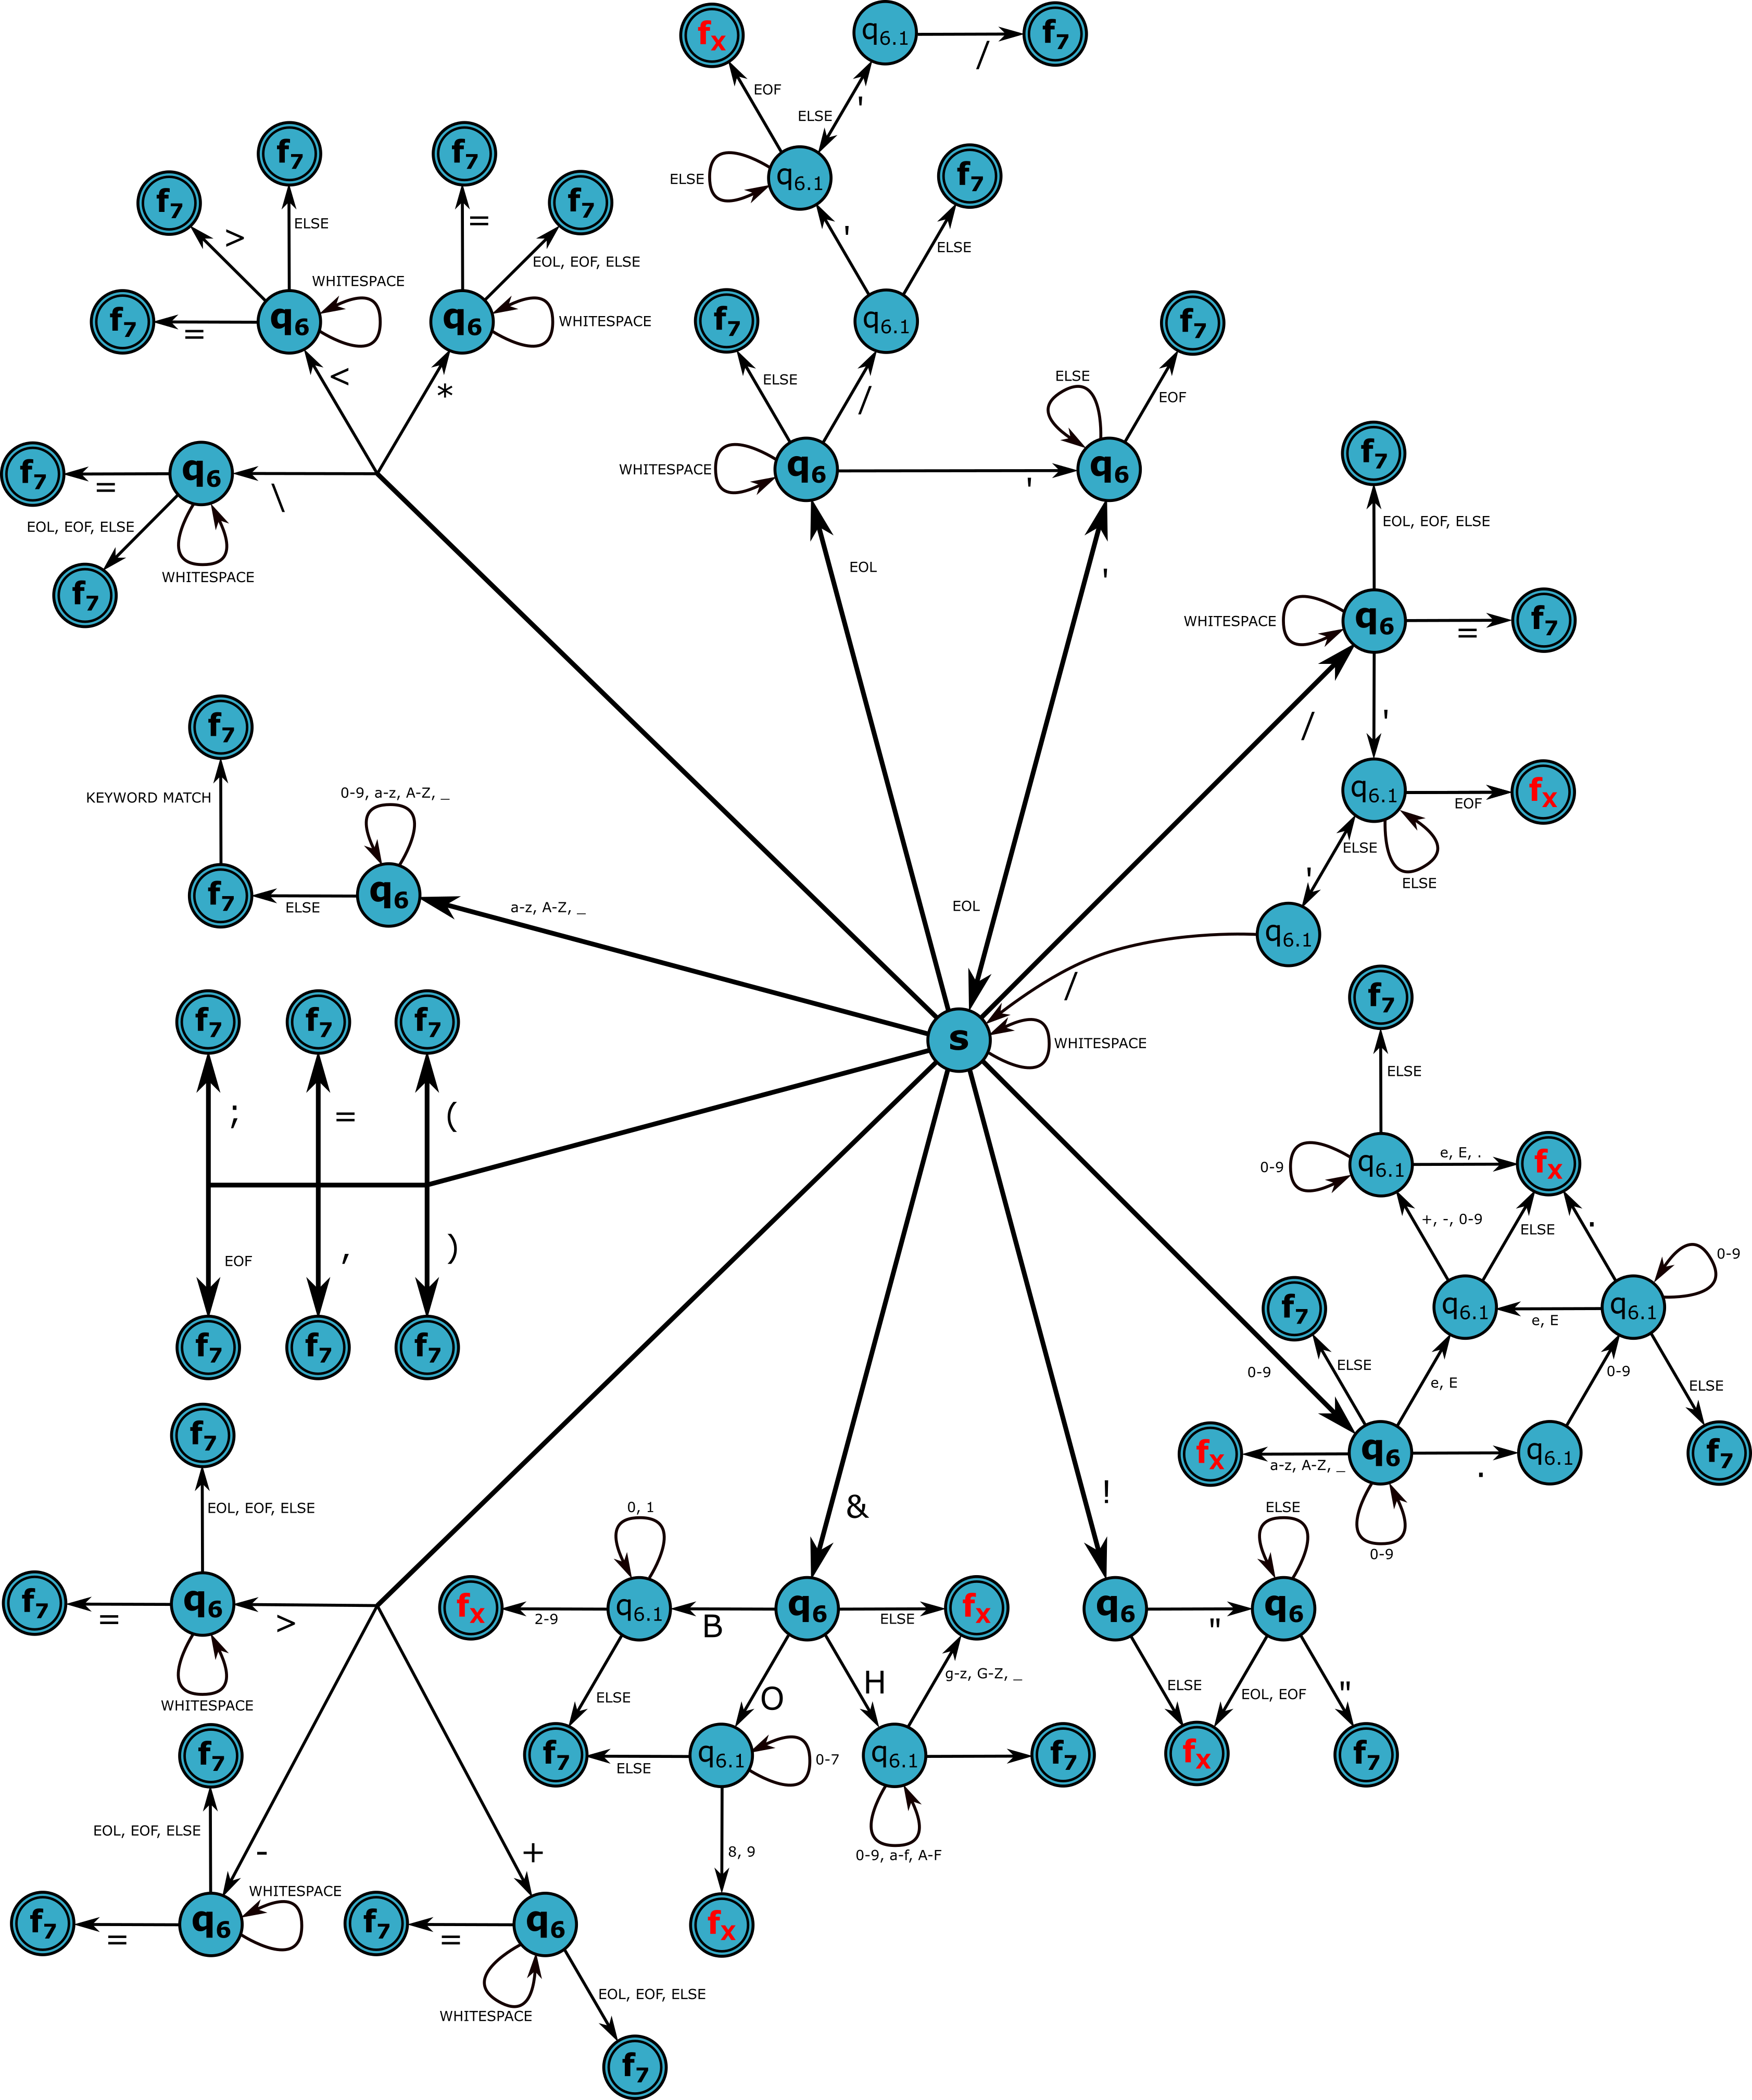
\includegraphics[height=20cm]{KA}}
    {\newpage}



    {\huge\bfseries Parser - Syntax \par}
    Implementoval xbartl06
    \vspace{1cm}

    {\scshape\Large Postup Implementace\par}
    \vspace{0.3cm}
    \noindent Hinzufügen den Text hier!
    \vspace{1cm}

    {\scshape\Large Funkce\par}
    \vspace{0.3cm}
    \noindent Hinzufügen den Text hier!
    \newpage



    {\huge\bfseries Parser - Sémantika \par}
    Implementoval xodehn08
    \vspace{1cm}

    {\scshape\Large Postup Implementace\par}
    \vspace{0.3cm}
    \noindent Hinzufügen den Text hier!
    \vspace{1cm}

    {\scshape\Large Funkce\par}
    \vspace{0.3cm}
    \noindent Hinzufügen den Text hier!
    \newpage



    {\huge\bfseries Generátor \par}
    Implementoval xsopfp00
    \vspace{1cm}

    {\scshape\Large Postup Implementace\par}
    \vspace{0.3cm}
    \noindent Hinzufügen den Text hier!
    \vspace{1cm}

    {\scshape\Large Funkce\par}
    \vspace{0.3cm}
    \noindent Hinzufügen den Text hier!
    \newpage
\end{document}